\documentclass[]{article}
\usepackage{lmodern}
\usepackage{amssymb,amsmath}
\usepackage{ifxetex,ifluatex}
\usepackage{fixltx2e} % provides \textsubscript
\ifnum 0\ifxetex 1\fi\ifluatex 1\fi=0 % if pdftex
  \usepackage[T1]{fontenc}
  \usepackage[utf8]{inputenc}
\else % if luatex or xelatex
  \ifxetex
    \usepackage{mathspec}
  \else
    \usepackage{fontspec}
  \fi
  \defaultfontfeatures{Ligatures=TeX,Scale=MatchLowercase}
\fi
% use upquote if available, for straight quotes in verbatim environments
\IfFileExists{upquote.sty}{\usepackage{upquote}}{}
% use microtype if available
\IfFileExists{microtype.sty}{%
\usepackage{microtype}
\UseMicrotypeSet[protrusion]{basicmath} % disable protrusion for tt fonts
}{}
\usepackage[margin=1in]{geometry}
\usepackage{hyperref}
\hypersetup{unicode=true,
            pdftitle={Homework 1 - Monte Carlo Methods},
            pdfauthor={Jared Garfinkel - jsg2145},
            pdfborder={0 0 0},
            breaklinks=true}
\urlstyle{same}  % don't use monospace font for urls
\usepackage{color}
\usepackage{fancyvrb}
\newcommand{\VerbBar}{|}
\newcommand{\VERB}{\Verb[commandchars=\\\{\}]}
\DefineVerbatimEnvironment{Highlighting}{Verbatim}{commandchars=\\\{\}}
% Add ',fontsize=\small' for more characters per line
\usepackage{framed}
\definecolor{shadecolor}{RGB}{248,248,248}
\newenvironment{Shaded}{\begin{snugshade}}{\end{snugshade}}
\newcommand{\AlertTok}[1]{\textcolor[rgb]{0.94,0.16,0.16}{#1}}
\newcommand{\AnnotationTok}[1]{\textcolor[rgb]{0.56,0.35,0.01}{\textbf{\textit{#1}}}}
\newcommand{\AttributeTok}[1]{\textcolor[rgb]{0.77,0.63,0.00}{#1}}
\newcommand{\BaseNTok}[1]{\textcolor[rgb]{0.00,0.00,0.81}{#1}}
\newcommand{\BuiltInTok}[1]{#1}
\newcommand{\CharTok}[1]{\textcolor[rgb]{0.31,0.60,0.02}{#1}}
\newcommand{\CommentTok}[1]{\textcolor[rgb]{0.56,0.35,0.01}{\textit{#1}}}
\newcommand{\CommentVarTok}[1]{\textcolor[rgb]{0.56,0.35,0.01}{\textbf{\textit{#1}}}}
\newcommand{\ConstantTok}[1]{\textcolor[rgb]{0.00,0.00,0.00}{#1}}
\newcommand{\ControlFlowTok}[1]{\textcolor[rgb]{0.13,0.29,0.53}{\textbf{#1}}}
\newcommand{\DataTypeTok}[1]{\textcolor[rgb]{0.13,0.29,0.53}{#1}}
\newcommand{\DecValTok}[1]{\textcolor[rgb]{0.00,0.00,0.81}{#1}}
\newcommand{\DocumentationTok}[1]{\textcolor[rgb]{0.56,0.35,0.01}{\textbf{\textit{#1}}}}
\newcommand{\ErrorTok}[1]{\textcolor[rgb]{0.64,0.00,0.00}{\textbf{#1}}}
\newcommand{\ExtensionTok}[1]{#1}
\newcommand{\FloatTok}[1]{\textcolor[rgb]{0.00,0.00,0.81}{#1}}
\newcommand{\FunctionTok}[1]{\textcolor[rgb]{0.00,0.00,0.00}{#1}}
\newcommand{\ImportTok}[1]{#1}
\newcommand{\InformationTok}[1]{\textcolor[rgb]{0.56,0.35,0.01}{\textbf{\textit{#1}}}}
\newcommand{\KeywordTok}[1]{\textcolor[rgb]{0.13,0.29,0.53}{\textbf{#1}}}
\newcommand{\NormalTok}[1]{#1}
\newcommand{\OperatorTok}[1]{\textcolor[rgb]{0.81,0.36,0.00}{\textbf{#1}}}
\newcommand{\OtherTok}[1]{\textcolor[rgb]{0.56,0.35,0.01}{#1}}
\newcommand{\PreprocessorTok}[1]{\textcolor[rgb]{0.56,0.35,0.01}{\textit{#1}}}
\newcommand{\RegionMarkerTok}[1]{#1}
\newcommand{\SpecialCharTok}[1]{\textcolor[rgb]{0.00,0.00,0.00}{#1}}
\newcommand{\SpecialStringTok}[1]{\textcolor[rgb]{0.31,0.60,0.02}{#1}}
\newcommand{\StringTok}[1]{\textcolor[rgb]{0.31,0.60,0.02}{#1}}
\newcommand{\VariableTok}[1]{\textcolor[rgb]{0.00,0.00,0.00}{#1}}
\newcommand{\VerbatimStringTok}[1]{\textcolor[rgb]{0.31,0.60,0.02}{#1}}
\newcommand{\WarningTok}[1]{\textcolor[rgb]{0.56,0.35,0.01}{\textbf{\textit{#1}}}}
\usepackage{graphicx,grffile}
\makeatletter
\def\maxwidth{\ifdim\Gin@nat@width>\linewidth\linewidth\else\Gin@nat@width\fi}
\def\maxheight{\ifdim\Gin@nat@height>\textheight\textheight\else\Gin@nat@height\fi}
\makeatother
% Scale images if necessary, so that they will not overflow the page
% margins by default, and it is still possible to overwrite the defaults
% using explicit options in \includegraphics[width, height, ...]{}
\setkeys{Gin}{width=\maxwidth,height=\maxheight,keepaspectratio}
\IfFileExists{parskip.sty}{%
\usepackage{parskip}
}{% else
\setlength{\parindent}{0pt}
\setlength{\parskip}{6pt plus 2pt minus 1pt}
}
\setlength{\emergencystretch}{3em}  % prevent overfull lines
\providecommand{\tightlist}{%
  \setlength{\itemsep}{0pt}\setlength{\parskip}{0pt}}
\setcounter{secnumdepth}{0}
% Redefines (sub)paragraphs to behave more like sections
\ifx\paragraph\undefined\else
\let\oldparagraph\paragraph
\renewcommand{\paragraph}[1]{\oldparagraph{#1}\mbox{}}
\fi
\ifx\subparagraph\undefined\else
\let\oldsubparagraph\subparagraph
\renewcommand{\subparagraph}[1]{\oldsubparagraph{#1}\mbox{}}
\fi

%%% Use protect on footnotes to avoid problems with footnotes in titles
\let\rmarkdownfootnote\footnote%
\def\footnote{\protect\rmarkdownfootnote}

%%% Change title format to be more compact
\usepackage{titling}

% Create subtitle command for use in maketitle
\providecommand{\subtitle}[1]{
  \posttitle{
    \begin{center}\large#1\end{center}
    }
}

\setlength{\droptitle}{-2em}

  \title{Homework 1 - Monte Carlo Methods}
    \pretitle{\vspace{\droptitle}\centering\huge}
  \posttitle{\par}
    \author{Jared Garfinkel - jsg2145}
    \preauthor{\centering\large\emph}
  \postauthor{\par}
    \date{}
    \predate{}\postdate{}
  

\begin{document}
\maketitle

\hypertarget{problem-1}{%
\section{Problem 1}\label{problem-1}}

The standard Laplace distribution has density
\[f(x) = 0.5e^{-|x|}, x \in
(-\infty, \infty)\]. Please provide an algorithm that uses the inverse
transformation method to generate a random sample from this
distribution. Use the \(U(0,1)\) random number generator in
\em{\bf{R}}, write a  \em{\bf{R}}-function to implement the algorithm. Use visualization tools to validate your algorithm (i.e., illustrate whether the random numbers generated from your function truely follows the standard Laplace distribution.)

\hypertarget{answer-your-answer-starts-here}{%
\section{Answer: your answer starts
here\ldots{}}\label{answer-your-answer-starts-here}}

X = \(F^{-1}(U)\)

\mu = \(F(x)\)

\(f(x) = 0.5e^{-|x|},~x \in(-\infty, \infty)\)

\begin{document}
\[   \left\{
\begin{array}{ll}
      F(x) = 0.5e^x & x \le 0 \\
      F(x) = 1-0.5e^{-x} & x > 0\\
\end{array} 
\right. \]
\end{document}

\begin{document}
\[   \left\{
\begin{array}{ll}
      x = ln(2U) & U < \frac{1}{2} \\
      x = -ln(2-2U) & U \ge \frac{1}{2}\\
\end{array} 
\right. \]
\end{document}

\begin{Shaded}
\begin{Highlighting}[]
\KeywordTok{set.seed}\NormalTok{(}\DecValTok{123}\NormalTok{)}
\NormalTok{U <-}\StringTok{ }\KeywordTok{runif}\NormalTok{(}\DecValTok{1000}\NormalTok{)}
\NormalTok{X <-}\StringTok{ }\NormalTok{(U }\OperatorTok{<}\StringTok{ }\FloatTok{0.5}\NormalTok{) }\OperatorTok{*}\StringTok{ }\KeywordTok{log}\NormalTok{(}\DecValTok{2}\OperatorTok{*}\NormalTok{U) }\OperatorTok{+}\StringTok{ }\NormalTok{(U }\OperatorTok{>=}\StringTok{ }\FloatTok{0.5}\NormalTok{) }\OperatorTok{*}\StringTok{ }\OperatorTok{-}\KeywordTok{log}\NormalTok{(}\DecValTok{2-2}\OperatorTok{*}\NormalTok{U)}

\KeywordTok{plot}\NormalTok{(X)}
\end{Highlighting}
\end{Shaded}

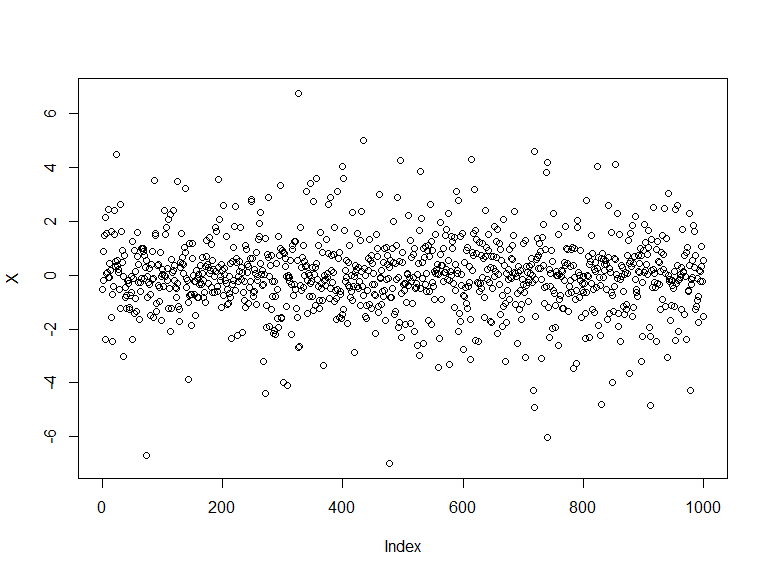
\includegraphics[width=0.9\linewidth]{homework-1---Monte-Carlo-Methods_files/figure-latex/unnamed-chunk-1-1}

\begin{Shaded}
\begin{Highlighting}[]
\KeywordTok{hist}\NormalTok{(X, }\DataTypeTok{prob =}\NormalTok{ T)}
\end{Highlighting}
\end{Shaded}

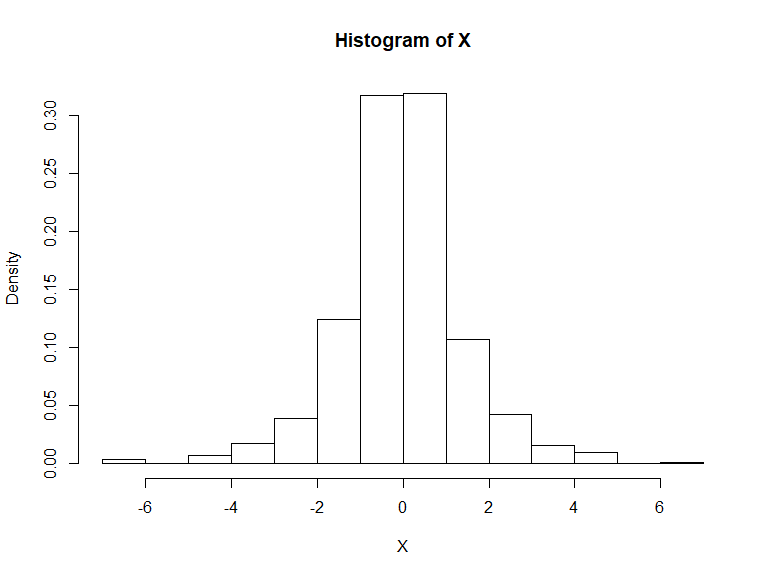
\includegraphics[width=0.9\linewidth]{homework-1---Monte-Carlo-Methods_files/figure-latex/unnamed-chunk-1-2}

\#Problem 2

Use the inverse transformation method to derive an algorithm for
generating a Pareto random number with \(U\sim U(0,1)\), where the
Pareto random number has a probability density function
\[f(x; \alpha, \gamma)=\frac{\gamma\alpha^{\gamma}}{x^{\gamma+1}} I\{x\ge \alpha\}\]
with two parameters \(\alpha >0\) and \(\gamma>0\). Use visualization
tools to validate your algorithm (i.e., illustrate whether the random
numbers generated from your function truely follows the target
distribution.)

\[F(x) = 1 - \left(\frac{\alpha}{x}\right)^{\gamma},~x \ge \alpha,~\alpha > 0,~\gamma > 0\]

\[x = \frac{\alpha}{(1-u)^{1/\gamma}}\]

\hypertarget{answer-your-answer-starts-here-1}{%
\section{Answer: your answer starts
here\ldots{}}\label{answer-your-answer-starts-here-1}}

\begin{Shaded}
\begin{Highlighting}[]
\KeywordTok{set.seed}\NormalTok{(}\DecValTok{1001}\NormalTok{)}
\NormalTok{U <-}\StringTok{ }\KeywordTok{runif}\NormalTok{(}\DecValTok{1000}\NormalTok{)}
\NormalTok{xdens =}\StringTok{ }\ControlFlowTok{function}\NormalTok{(}\DataTypeTok{gamma =} \DecValTok{5}\NormalTok{, }\DataTypeTok{alpha =} \DecValTok{2}\NormalTok{, }\DataTypeTok{x =}\NormalTok{ U) \{}
\NormalTok{  alpha}\OperatorTok{/}\NormalTok{((}\DecValTok{1}\OperatorTok{-}\NormalTok{U)}\OperatorTok{^}\NormalTok{(}\DecValTok{1}\OperatorTok{/}\NormalTok{gamma))}
\NormalTok{\}}

\NormalTok{x <-}\StringTok{ }\KeywordTok{xdens}\NormalTok{(}\DecValTok{5}\NormalTok{, }\DecValTok{2}\NormalTok{, U)}

\KeywordTok{hist}\NormalTok{(x, }\DataTypeTok{prob =}\NormalTok{ T)}
\end{Highlighting}
\end{Shaded}

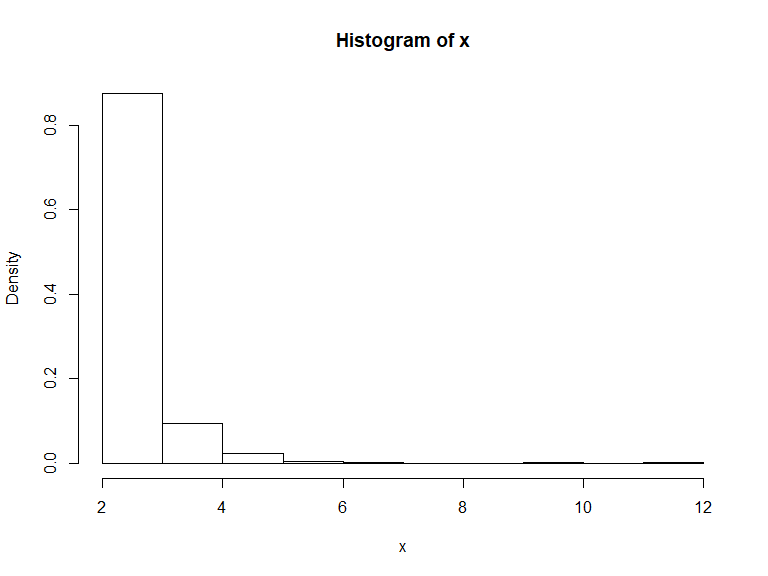
\includegraphics[width=0.9\linewidth]{homework-1---Monte-Carlo-Methods_files/figure-latex/unnamed-chunk-2-1}

\#Problem 3

Construct an algorithm for using the acceptance/rejection method to
generate 100 pseudorandom variable from the pdf
\[f(x) = \frac{2}{\pi \beta^2} \sqrt{\beta^2-x^2}, \,\, -\beta \le x \le \beta.\]
The simplest choice for \(g(x)\) is the \(U(-\beta, \beta)\)
distribution but other choices are possible as well. Use visualization
tools to validate your algorithm (i.e., illustrate whether the random
numbers generated from your function truely follows the target
distribution.)

\hypertarget{answer-your-answer-starts-here-2}{%
\section{Answer: your answer starts
here\ldots{}}\label{answer-your-answer-starts-here-2}}

\begin{Shaded}
\begin{Highlighting}[]
\KeywordTok{set.seed}\NormalTok{(}\DecValTok{1001}\NormalTok{)}

\NormalTok{accrej <-}\StringTok{ }\ControlFlowTok{function}\NormalTok{(fdens, gdens, beta, }\DataTypeTok{M =}\NormalTok{ (}\DecValTok{4}\OperatorTok{/}\NormalTok{pi), x)\{}
\NormalTok{  x =}\StringTok{ }\KeywordTok{runif}\NormalTok{(}\DecValTok{100}\NormalTok{, }\DataTypeTok{min =} \OperatorTok{-}\NormalTok{beta, }\DataTypeTok{max =}\NormalTok{ beta)}
  \KeywordTok{return}\NormalTok{(x[}\KeywordTok{runif}\NormalTok{(}\KeywordTok{length}\NormalTok{(x)) }\OperatorTok{<=}\StringTok{ }\KeywordTok{fdens}\NormalTok{(x, beta) }\OperatorTok{/}\StringTok{ }\NormalTok{(M }\OperatorTok{*}\StringTok{ }\KeywordTok{gdens}\NormalTok{(x, beta))])}
\NormalTok{\}}

\NormalTok{xdens =}\StringTok{ }\ControlFlowTok{function}\NormalTok{(x, beta)\{}
  \KeywordTok{return}\NormalTok{((}\DecValTok{2}\OperatorTok{/}\NormalTok{(pi}\OperatorTok{*}\NormalTok{beta}\OperatorTok{^}\DecValTok{2}\NormalTok{))}\OperatorTok{*}\KeywordTok{sqrt}\NormalTok{(beta}\OperatorTok{^}\DecValTok{2} \OperatorTok{-}\StringTok{ }\NormalTok{x}\OperatorTok{^}\DecValTok{2}\NormalTok{) }\OperatorTok{*}\StringTok{ }\NormalTok{(}\KeywordTok{abs}\NormalTok{(x) }\OperatorTok{<=}\StringTok{ }\NormalTok{beta))}
\NormalTok{\}}

\NormalTok{unifdens =}\StringTok{ }\ControlFlowTok{function}\NormalTok{(x, beta)\{}
  \KeywordTok{return}\NormalTok{((}\DecValTok{1}\OperatorTok{/}\NormalTok{(}\DecValTok{2}\OperatorTok{*}\NormalTok{beta))}\OperatorTok{*}\NormalTok{(}\KeywordTok{abs}\NormalTok{(x) }\OperatorTok{<=}\StringTok{ }\NormalTok{beta))}
\NormalTok{\}}


\NormalTok{y =}\StringTok{ }\KeywordTok{accrej}\NormalTok{(xdens, unifdens, }\DecValTok{3}\NormalTok{, }\DecValTok{4}\OperatorTok{/}\NormalTok{pi)}

\KeywordTok{hist}\NormalTok{(y, }\DataTypeTok{prob =}\NormalTok{ T)}
\end{Highlighting}
\end{Shaded}

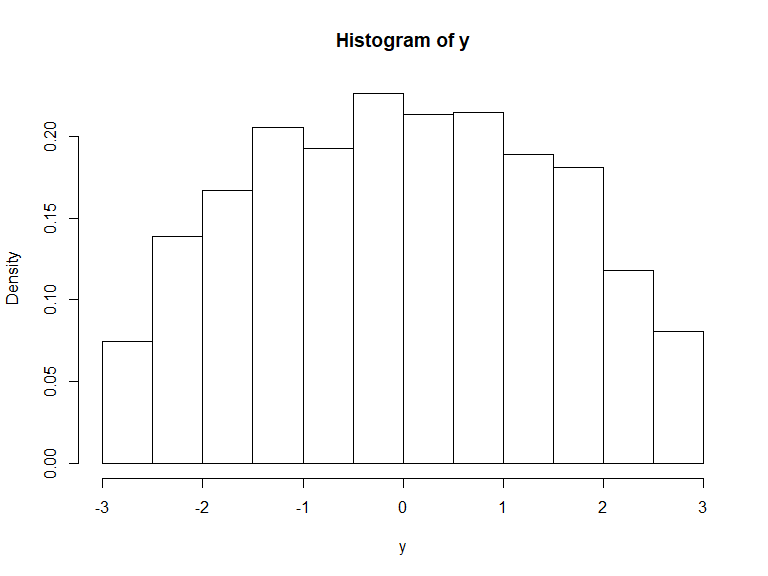
\includegraphics[width=0.9\linewidth]{homework-1---Monte-Carlo-Methods_files/figure-latex/unnamed-chunk-3-1}

\#Problem 4

Develop two Monte Carlo methods for the estimation of
\(\theta=\int_0^1 e^{x^2} dx\) and implement in \em{\bf{R}} .

\hypertarget{answer-your-answer-starts-here-3}{%
\section{Answer: your answer starts
here\ldots{}}\label{answer-your-answer-starts-here-3}}

\begin{Shaded}
\begin{Highlighting}[]
\NormalTok{n =}\StringTok{ }\DecValTok{10000}
\NormalTok{u =}\StringTok{ }\KeywordTok{runif}\NormalTok{(n)}
\NormalTok{y =}\StringTok{ }\KeywordTok{sum}\NormalTok{(}\KeywordTok{exp}\NormalTok{(u}\OperatorTok{^}\DecValTok{2}\NormalTok{))}\OperatorTok{/}\NormalTok{n}
\NormalTok{x =}\StringTok{ }\KeywordTok{median}\NormalTok{(}\KeywordTok{exp}\NormalTok{(u}\OperatorTok{^}\DecValTok{2}\NormalTok{))}

\NormalTok{xy =}\StringTok{ }\KeywordTok{tibble}\NormalTok{(}
  \DataTypeTok{median =}\NormalTok{ x,}
  \DataTypeTok{mean =}\NormalTok{ y}
\NormalTok{) }\OperatorTok\StringTok{ }
\StringTok{  }\NormalTok{knitr}\OperatorTok{::}\KeywordTok{kable}\NormalTok{()}
\end{Highlighting}
\end{Shaded}

\#Problem 5

Show that in estimating \(\theta=E\sqrt{1-U^2}\) it is better to use
\(U^2\) rather than \(U\) as the control variate, where
\(U\sim U(0,1)\). To do this, use simulation to approximate the
necessary covariances. In addition, implement your algorithms in
\em{\bf{R}}.

\hypertarget{using-u2-the-variance-is-lower-than-using-u-as-the-control-variate}{%
\subsection{Using U\^{}2 the variance is lower than using U as the
control
variate}\label{using-u2-the-variance-is-lower-than-using-u-as-the-control-variate}}

The variance is lower for u\^{}2 (-4.43) than for u (-4.09) as the
control variate as shown below.

\begin{Shaded}
\begin{Highlighting}[]
\NormalTok{gfun<-}\ControlFlowTok{function}\NormalTok{(x)\{ }
  \KeywordTok{sqrt}\NormalTok{(}\DecValTok{1} \OperatorTok{-}\StringTok{ }\NormalTok{x}\OperatorTok{^}\DecValTok{2}\NormalTok{)}
\NormalTok{\}}
\NormalTok{mfun<-}\ControlFlowTok{function}\NormalTok{(x) \{}
\NormalTok{  x}\OperatorTok{^}\DecValTok{2}
\NormalTok{\}}
\NormalTok{mfun2<-}\ControlFlowTok{function}\NormalTok{(x) \{}
\NormalTok{  x}
\NormalTok{\}}
\KeywordTok{set.seed}\NormalTok{(}\DecValTok{123}\NormalTok{)}
\NormalTok{uran<-}\KeywordTok{runif}\NormalTok{(}\DecValTok{10000}\NormalTok{)}
\NormalTok{ga<-}\KeywordTok{gfun}\NormalTok{(uran)}
\NormalTok{ma<-}\KeywordTok{mfun}\NormalTok{(uran)}
\NormalTok{ma2<-}\KeywordTok{mfun2}\NormalTok{(uran)}
\end{Highlighting}
\end{Shaded}

\begin{Shaded}
\begin{Highlighting}[]
\NormalTok{theta1<-}\KeywordTok{mean}\NormalTok{(ga)}
\NormalTok{theta2<-}\KeywordTok{mean}\NormalTok{(ma2)}
\NormalTok{hha<-}\StringTok{ }\NormalTok{pi}\OperatorTok{/}\DecValTok{4} \OperatorTok{+}\StringTok{ }\NormalTok{(ga}\OperatorTok{-}\NormalTok{ma)}
\NormalTok{hha2<-}\StringTok{ }\NormalTok{pi}\OperatorTok{/}\DecValTok{4} \OperatorTok{+}\StringTok{ }\NormalTok{(ga}\OperatorTok{-}\NormalTok{ma2)}
\NormalTok{theta1a<-}\KeywordTok{mean}\NormalTok{(hha)}
\NormalTok{theta2a<-}\KeywordTok{mean}\NormalTok{(hha2)}

\KeywordTok{c}\NormalTok{(}\KeywordTok{var}\NormalTok{(ga), }\KeywordTok{var}\NormalTok{(hha))}
\end{Highlighting}
\end{Shaded}

\begin{verbatim}
## [1] 0.04848323 0.26344282
\end{verbatim}

\begin{Shaded}
\begin{Highlighting}[]
\KeywordTok{c}\NormalTok{(}\KeywordTok{var}\NormalTok{(ga), }\KeywordTok{var}\NormalTok{(hha2))}
\end{Highlighting}
\end{Shaded}

\begin{verbatim}
## [1] 0.04848323 0.24693579
\end{verbatim}

\begin{Shaded}
\begin{Highlighting}[]
\NormalTok{(}\KeywordTok{var}\NormalTok{(ga)}\OperatorTok{-}\KeywordTok{var}\NormalTok{(hha))}\OperatorTok{/}\KeywordTok{var}\NormalTok{(ga)}
\end{Highlighting}
\end{Shaded}

\begin{verbatim}
## [1] -4.43369
\end{verbatim}

\begin{Shaded}
\begin{Highlighting}[]
\NormalTok{(}\KeywordTok{var}\NormalTok{(ga)}\OperatorTok{-}\KeywordTok{var}\NormalTok{(hha2))}\OperatorTok{/}\KeywordTok{var}\NormalTok{(ga)}
\end{Highlighting}
\end{Shaded}

\begin{verbatim}
## [1] -4.093221
\end{verbatim}

\#Problem 6 Obtain a Monte Carlo estimate of
\[\int_1^\infty \frac{x^2}{\sqrt{2\pi}} e^{-\frac{x^2}{2}} dx\] by
importance sampling and evaluate its variance. Write a
\em{\bf{R}} function to implement your procedure.

\hypertarget{use-a-normal-distribution-to-implement-importance-sampling-on-the-function-above.}{%
\subsection{Use a normal distribution to implement importance sampling
on the function
above.}\label{use-a-normal-distribution-to-implement-importance-sampling-on-the-function-above.}}

I generated a random sample of a uniform distribution from 0 to 1.

\begin{Shaded}
\begin{Highlighting}[]
\NormalTok{ncandidates <-}\StringTok{ }\DecValTok{100000}\NormalTok{;  }
\NormalTok{M <-}\StringTok{ }\KeywordTok{exp}\NormalTok{(}\OperatorTok{-}\DecValTok{1}\NormalTok{)}
\NormalTok{u =}\StringTok{ }\KeywordTok{runif}\NormalTok{(ncandidates)}
\NormalTok{x <-}\StringTok{ }\KeywordTok{rnorm}\NormalTok{(ncandidates)}
\NormalTok{Mfun <-}\StringTok{ }\ControlFlowTok{function}\NormalTok{(x)\{}
\NormalTok{  x}\OperatorTok{^}\DecValTok{2}\OperatorTok{*}\KeywordTok{exp}\NormalTok{(}\OperatorTok{-}\NormalTok{x}\OperatorTok{^}\DecValTok{2}\OperatorTok{/}\DecValTok{2}\NormalTok{)}\OperatorTok{/}\KeywordTok{sqrt}\NormalTok{(}\DecValTok{2}\OperatorTok{*}\NormalTok{pi)}
\NormalTok{\}}
\NormalTok{pfun <-}\StringTok{ }\ControlFlowTok{function}\NormalTok{(x)\{}
  \KeywordTok{dnorm}\NormalTok{(x)}
\NormalTok{\}}
\NormalTok{accrej <-}\StringTok{ }\ControlFlowTok{function}\NormalTok{(Mfun, pfun, M, x)\{}
\NormalTok{  ncandidates =}\StringTok{ }\KeywordTok{length}\NormalTok{(x)}
\NormalTok{  u =}\StringTok{ }\KeywordTok{rexp}\NormalTok{(ncandidates)}
\NormalTok{  accepted <-}\StringTok{ }\OtherTok{NULL}      \CommentTok{# Initialize the vector of accepted values}
  \ControlFlowTok{for}\NormalTok{(i }\ControlFlowTok{in} \DecValTok{1}\OperatorTok{:}\NormalTok{ncandidates) \{}
    \ControlFlowTok{if}\NormalTok{(u[i] }\OperatorTok{<=}\StringTok{ }\KeywordTok{Mfun}\NormalTok{(x[i])}\OperatorTok{/}\NormalTok{(M}\OperatorTok{*}\KeywordTok{pfun}\NormalTok{(x[i])))}
\NormalTok{      accepted <-}\StringTok{ }\KeywordTok{c}\NormalTok{(accepted, x[i])  }\CommentTok{# Accept x[i]}
\NormalTok{  \}}
  \KeywordTok{return}\NormalTok{(accepted)}
\NormalTok{\}}

\NormalTok{y =}\StringTok{ }\KeywordTok{accrej}\NormalTok{(Mfun, pfun, }\DecValTok{1}\OperatorTok{/}\KeywordTok{exp}\NormalTok{(}\DecValTok{1}\NormalTok{), x)}

\KeywordTok{hist}\NormalTok{(u)}
\KeywordTok{hist}\NormalTok{(y, }\DataTypeTok{prob =}\NormalTok{ T)}

\KeywordTok{sum}\NormalTok{(y}\OperatorTok{*}\NormalTok{(y}\OperatorTok{>}\DecValTok{1}\NormalTok{))}\OperatorTok{/}\KeywordTok{length}\NormalTok{(y}\OperatorTok{*}\NormalTok{(y}\OperatorTok{>}\DecValTok{1}\NormalTok{))}
\end{Highlighting}
\end{Shaded}


\end{document}
